% !TEX root = /home/weznon/programming/0207Programming/ftc-guides/programming/main.tex

\documentclass[../main.tex]{subfiles}

\begin{document}
\newpage
%Begin the stuff!
%This version of the template has some placeholder stuff so you can see what it looks like
\part{Vision}
While this really should go under sensors, it is a big enough category to warrant a section for itself.

\section{What is it}
We have previously discussed various sensors. However, the limitation inherent with all of them is the fact that they are all highly specialized with specific target ranges. The primary advantage of vision systems is that they offer a much larger range of view.
\section{OK but why do I need it}
\section{Vuforia}
\section{PixyCam}
\begin{figure}[H]
    \centering
    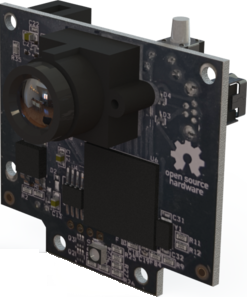
\includegraphics{sections/vision/images/pixy.png}
    \caption{A PixyCam, so you know what it looks like.}
\end{figure}
PixyCam is another vision system. It provides object recognizing capability by grouping together various pixels of a similar color. The color, thresholds, etc. can be set using a program you install on your computer. The main takeaway from this is that the Pixy is best suited to identifying objects of a roughly uniform color, based on the presence of that color in the image it sees.

TOOD: Insert some pictures of the training thing here. Requires using a pixy

We do not have example code for using a PixyCam, since we have never used it on our robot. This is for a couple of reasons. The first of which is that PixyCam is INCREDIBLY susceptible to lighting changes. It is highly likely that on competition day your settings will not work, depending on the lighting conditions at the meet. The second is that even when under proper settings, it isn't that great. It uses RGB, which is not the greatest for color detection. It has tons of false positives and noise, and all around isn't great. It works best on bright colors - the particles/jewels from Velocity Vortex/Relic Recovery, the relic from Relic Recovery, and the gold mineral from Rover Ruckus would work well. The glyphs from Relic Recovery worked horribly. 

\subsection{TL;DR}
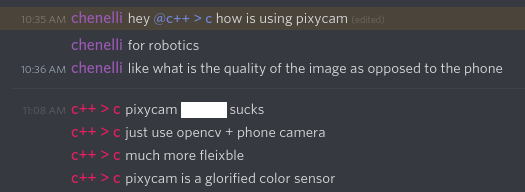
\includegraphics[width=400pt]{sections/vision/images/2019-02-27-195334_3840x1080_scrot_cropped.png}

\section{Tensorflow}
Tensorflow is an interesting vision system. The premise is this; there is some neural network trained to identify different pieces present in the game. This was first done in the Rover Ruckus season, as since I am currently writing this while that season takes place, I don't know whether it will be done again, as FTC trained the model to detect the minerals themselves. It is something you could do yourself, see subsection 3.6 DIY Neural Network. 
\begin{figure}[H]
    \centering
    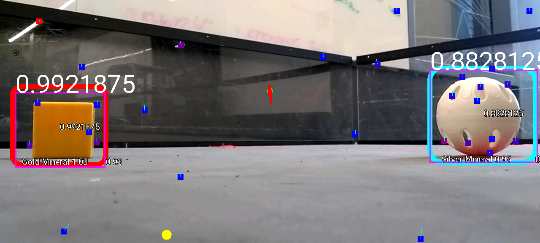
\includegraphics[width=400pt]{sections/vision/images/tensorflowOutput.png}
    \caption{Sample output of the Tensorflow. Each object that it believes to be a trained object, in this case the minerals, is boxed. Next to each box is a number, representing how confident the neural network is that the box is a mineral. In the FTC SDK, methods for getting the location of the box, confidence, and type of identified object the box contains are exposed}
\end{figure}

So, what does this look like from a programming standpoint? A full teleop which implements the Tensorflow identification (at least for the 2018-2019 season) can be found in TODO: figure out appendixes.

For now, assume that \verb|tfod| is a standard Tensorflow object provided by the FTC SDK.

\begin{lstlisting}[language=Java]
\end{lstlisting}

\section{DIY Neural Network}
A quick disclaimer before we get into this section, this will method for vision will take a long time (and if you do not have a GPU, even longer), so only use it if nothing is working. It requires a lot of patience and a lot of StackOverflow tabs to be opened, but if you really want to do it go for it. In order to train, you need to atleast have python installed.

The specific algorithm you will have to use is called YOLO object detection. In short, it takes in continuous video and splits the frame into a bunch of little rectangles and trys to find whatever you are looking for in those little rectangles. If it finds it, it'll but an little box around it. 

The first part of this method is to find find and annotate your dataset. Look around the internet or take some pictures and start to gather a dataset. Once you have your data, you have to start annotating. In order to annotate these images, you will need to use LabelImg. LabelImg makes the annotations in a way that the neural network can understand it (a.k.a. makes xml files). You can find LabelImg  \href{https://github.com/tzutalin/labelImg}{here}.

\begin{figure}[H]
    \centering
    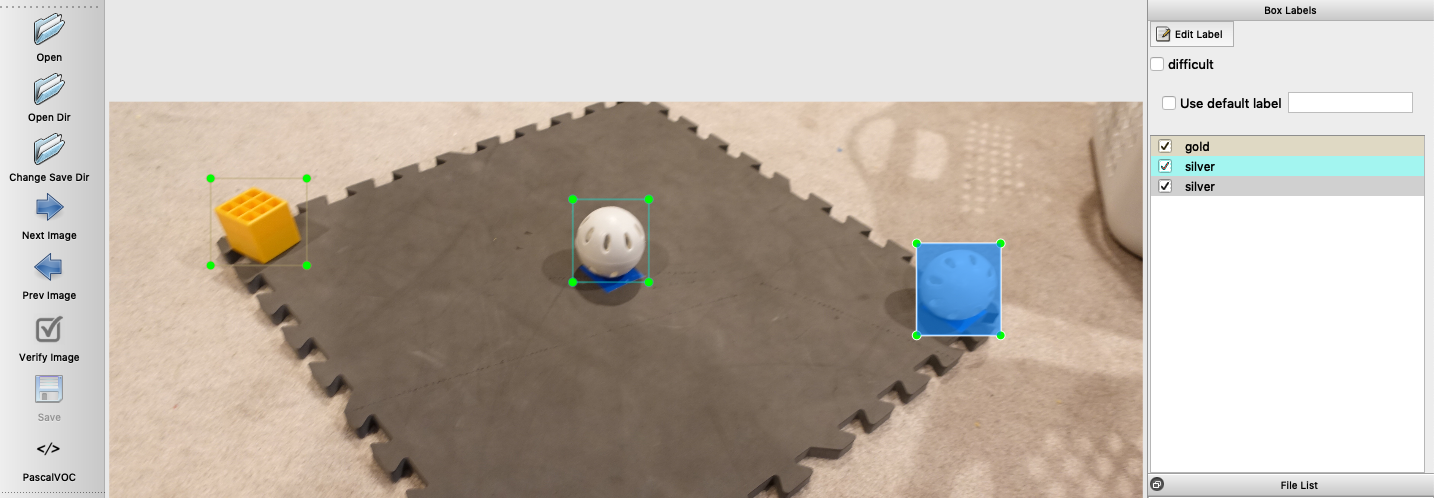
\includegraphics[width=400pt]{sections/vision/images/LabelImg.png}
    \caption{Sample screencap of labelling the images.}
\end{figure}

\section{OpenCV}
\subsection{Overview}
Computer Vision is the field of getting data from images that a computer can use. While the aforementioned TensorFlow does count in this regard as Computer Vision, typically Computer Vision refers to more direct algorithms - not trained neural nets. OpenCV is a collection of the various algorithms people have developed for various languages, including java. OpenCV allows for a much more flexible method of detecting and classifying objects in an FTC game.

The algorithms, or operations, provided by OpenCV can be chained together into a pipeline. To this pipeline an image is fed in, and out some information about that image is returned. Thus, when developing an OpenCV pipeline, one will first want to experiment with different operations to perform the desired action.
\subsection{GRIP}
Provided by WPI and found at \url{https://github.com/WPIRoboticsProjects/GRIP/}, GRIP is an extremely useful program for creating an OpenCV pipeline\footnote{A short tutorial on how to use GRIP can be found at \url{https://wpilib.screenstepslive.com/s/currentCS/m/vision/l/463566-introduction-to-grip}}.
\subsection{Operations}
\subsubsection{Image Resizing}
This operation is pretty self explanatory. The input image from the phone is resized. There are a bunch of methods of interpolation - how the computer knows what colors to make the pixels in the new image - but you can keep this on the default, cubic, since it really doesn't have much of an effect\footnote{You typically end up messing up the image with a blur, erosion, or dilation, so any work the phone does to interpolate data will be destroyed.}. The importance of this step is to decrease the size of the image, allowing following operations to run must faster - if there is less image to look at, less time is needed.
\begin{figure}[H]
    \centering
    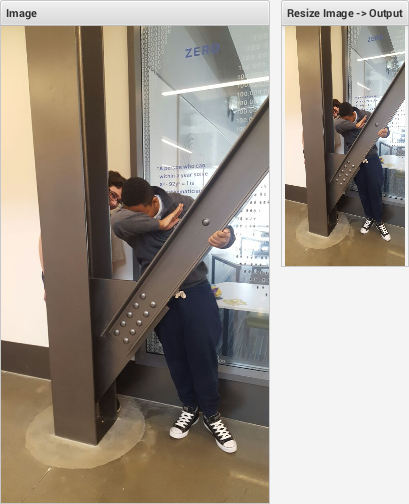
\includegraphics[height=200pt]{sections/vision/images/opencv/crawley/crawleyResize.png}
    \caption{Resized picture of Crawley dabbing in GRIP}
\end{figure}
\subsubsection{Color Converting}
make sure to mention caveat about the HSV on phones
\begin{figure}[H]
    \centering
    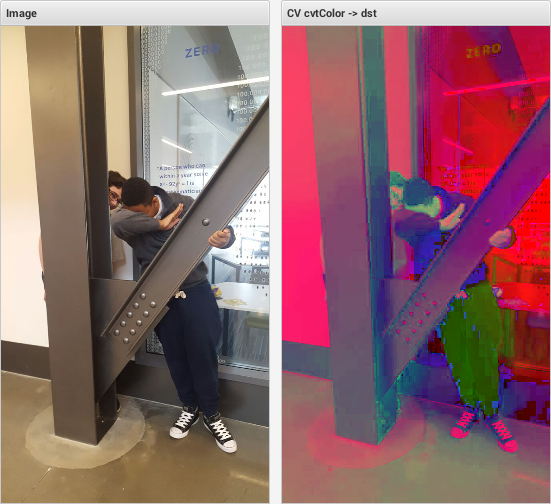
\includegraphics[height=200pt]{sections/vision/images/opencv/crawley/crawleyHSVTransform.png}
    \caption{RGB Image of Crawley converted to HSV color space in GRIP}
\end{figure}

\subsubsection{Blurring}
\begin{figure}[H]
    \centering
    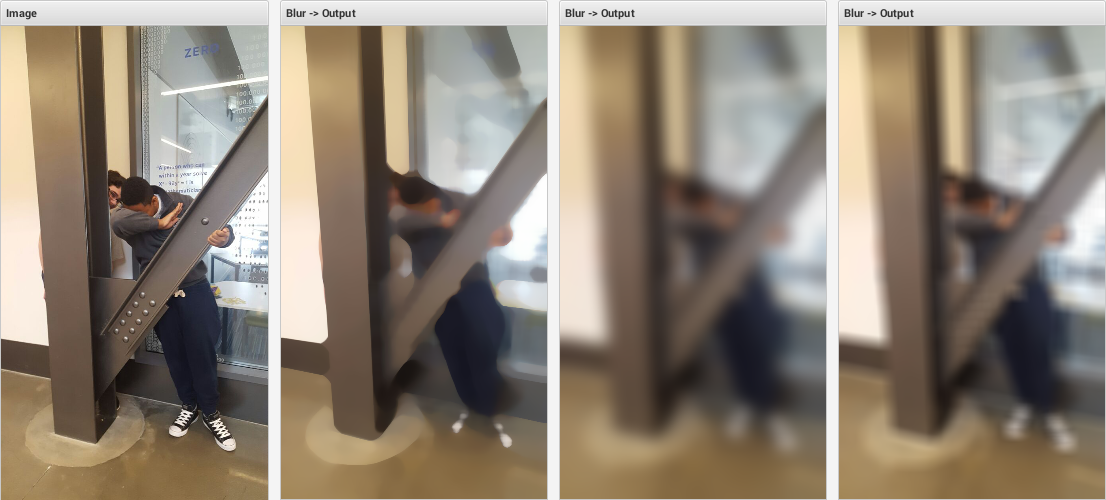
\includegraphics[height=200pt]{sections/vision/images/opencv/crawley/crawleyBlursMedianGaussianBox.png}
    \caption{3 types of blurs (Median, Gaussian, Box, in that order) on Crawley}
\end{figure}

\subsubsection{Erosion}
\begin{figure}[H]
    \centering
    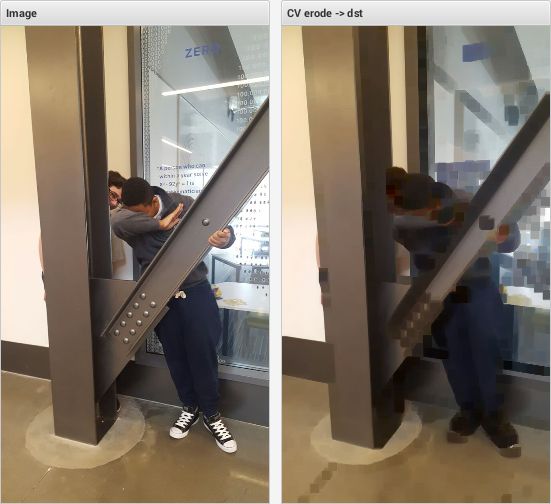
\includegraphics[height=200pt]{sections/vision/images/opencv/crawley/crawleyErode.png}
    \caption{Heavily eroded image of Crawley}
\end{figure}

\subsubsection{Dilation}
\begin{figure}[H]
    \centering
    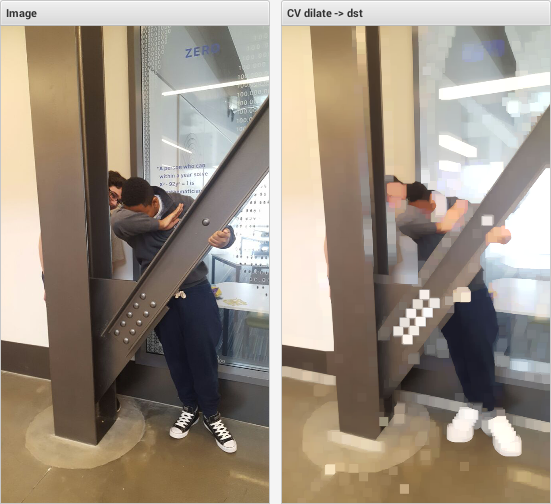
\includegraphics[height=200pt]{sections/vision/images/opencv/crawley/crawleyDilate.png}
    \caption{Heavily dilated image of Crawley}
\end{figure}
\subsubsection{Color Thresholding}
\begin{figure}[H]
    \centering
    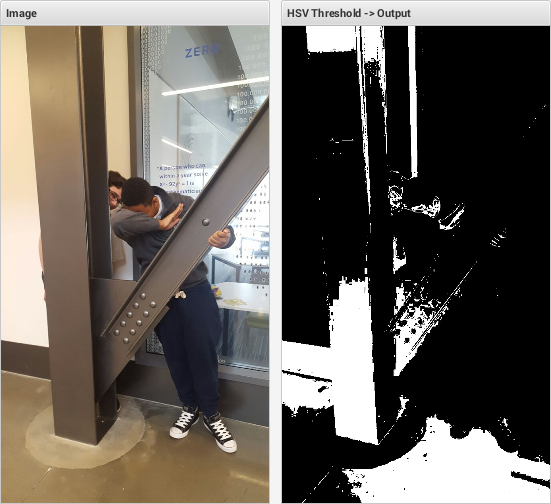
\includegraphics[height=200pt]{sections/vision/images/opencv/crawley/crawleyRandomThreshold.png}
    \caption{Meaningless thresholding of image of Crawley}
\end{figure}
\subsubsection{Finding Contours}
\begin{figure}[H]
    \centering
    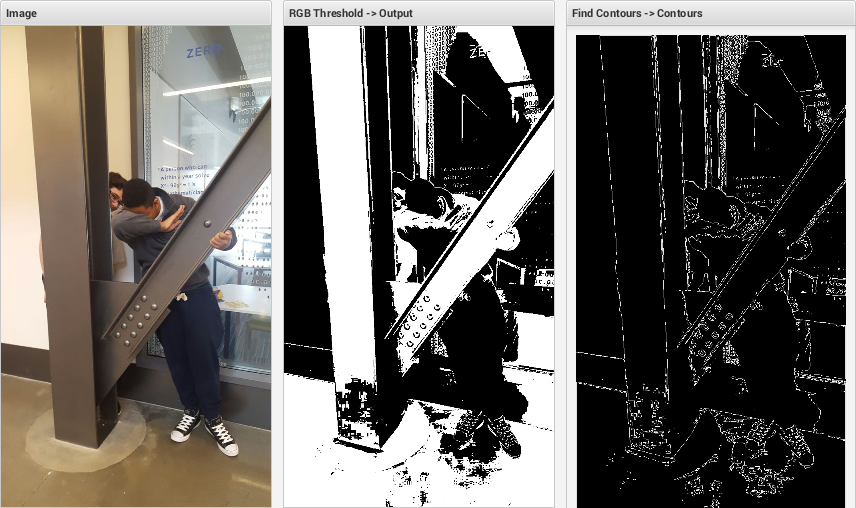
\includegraphics[height=200pt]{sections/vision/images/opencv/crawley/crawleyContour.png}
    \caption{Various contours in another pretty meaningless thresholding of the image of Crawley}
\end{figure}
\subsubsection{Finding Blobs}
\begin{figure}[H]
    \centering
    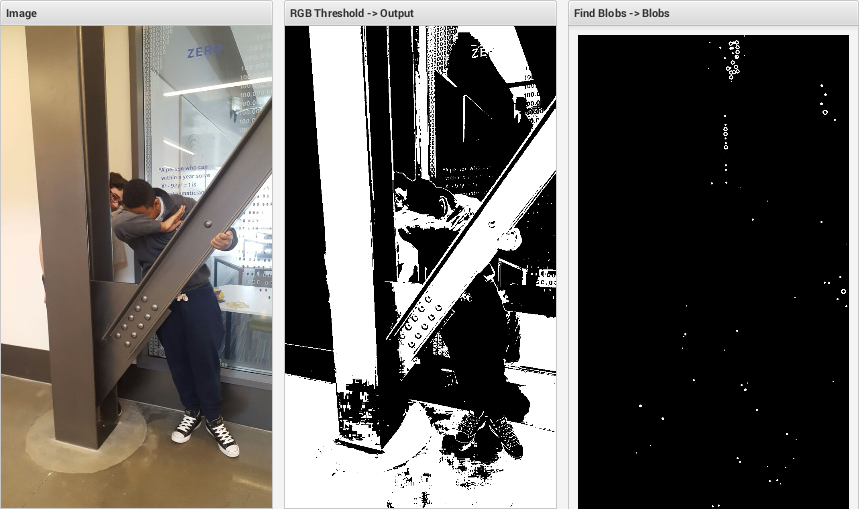
\includegraphics[height=200pt]{sections/vision/images/opencv/crawley/crawleyBlob.png}
    \caption{Failed attempt at finding blobs in an image that is not properly thresholded for finding blobs}
\end{figure}
\subsection{Example Pipelines}
\subsubsection{Gold Mineral Location Detection for Sampling in Rover Ruckus}
This pipeline is the (nearly) exact pipeline 207 used at NJ states in the Rover Ruckus season, with much success. First, a demonstration of the final product.
\begin{figure}[H]
    \centering
    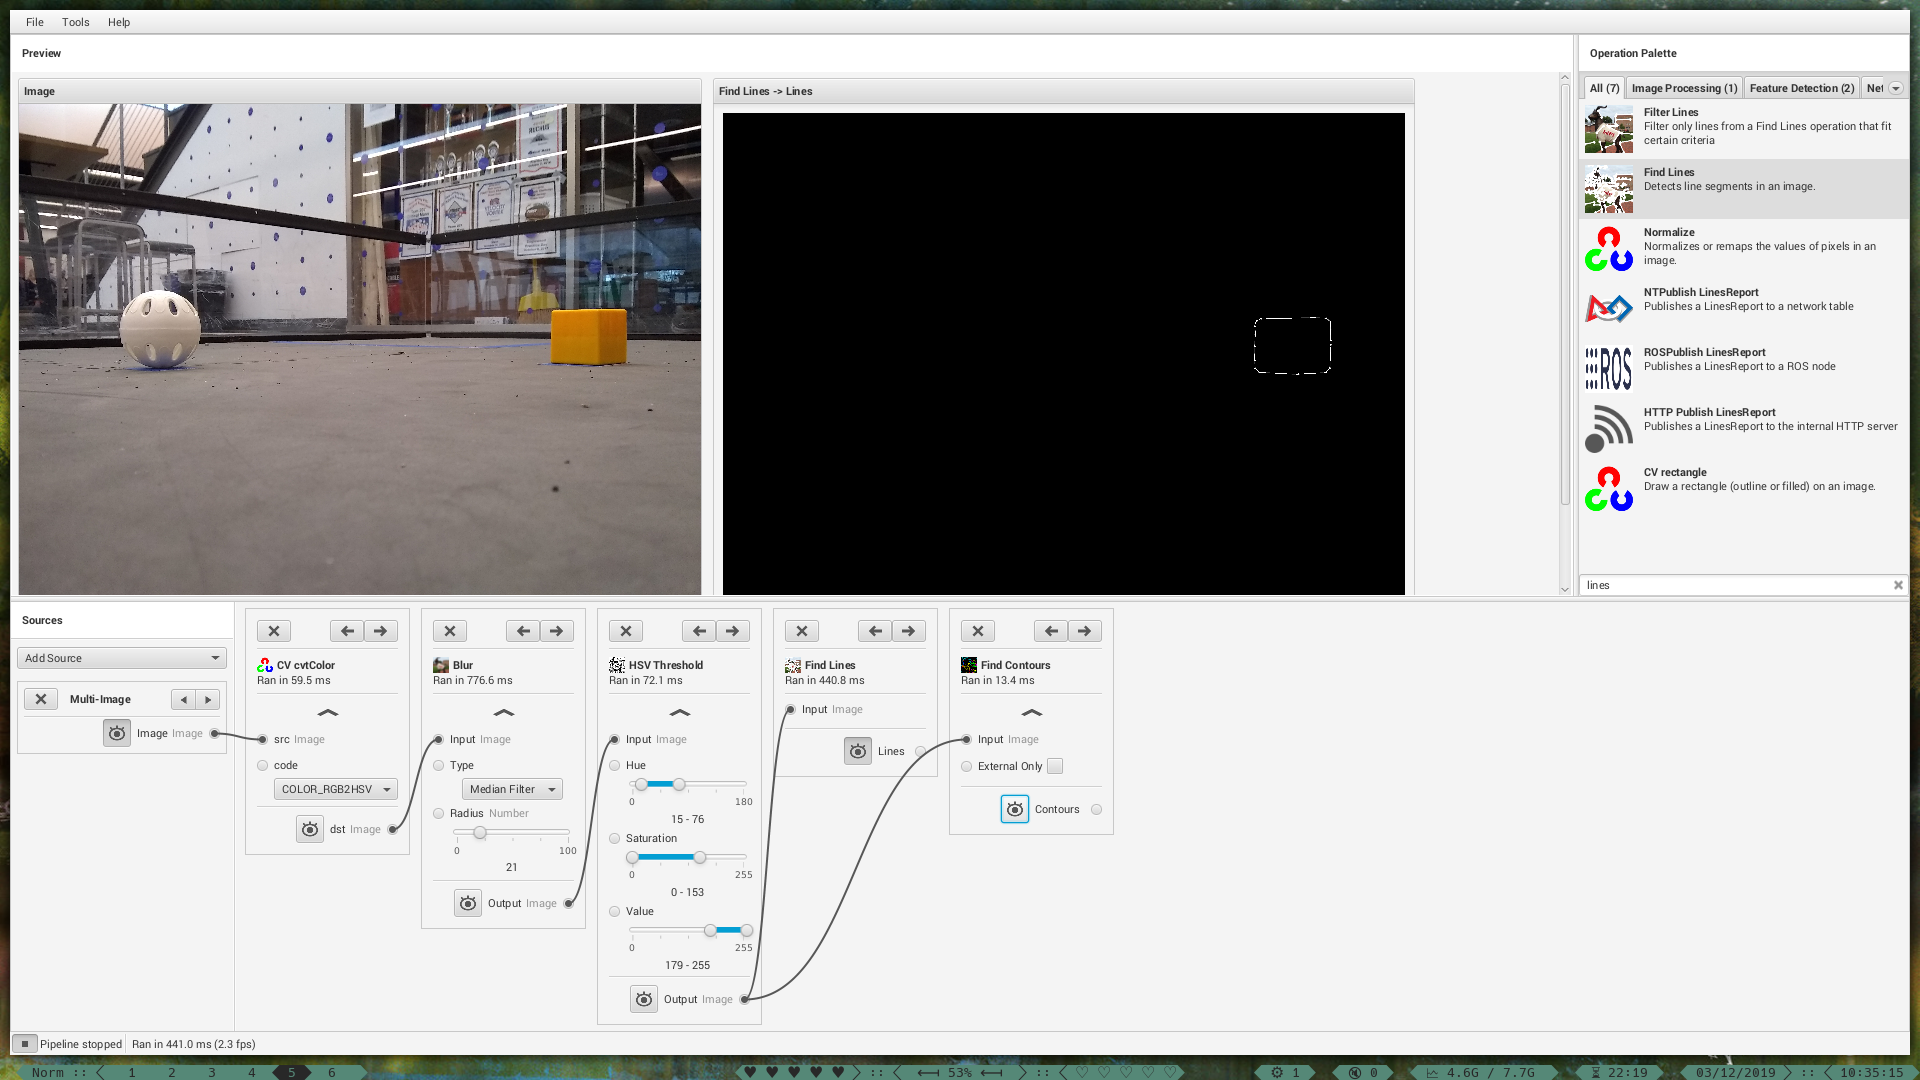
\includegraphics[width=400pt]{sections/vision/images/opencv/gold_grip_screenshot.png}
    \caption{The white box is the location of the gold mineral the code can use. This is using a line detection algorithm, as the result from that is easier to see - contour gives a very faint line. The identified location is exactly the same, however. I have also forgone the resizing step since the images are then too small to see clearly.}
\end{figure}
So, having shown that it works for at least one case, let's go over how the pipeline was made and works. The first (omitted in the example) step is to resize the image. We do this because we do not need a whole lot of detailin our detection - we only really care about the two big mineral pixel areas. Thus, by resizing, we can speed up our identification, with no detriment to the algorithm efficacy. The next step is to convert the image color space to HSV. 
\begin{figure}[H]
    \centering
    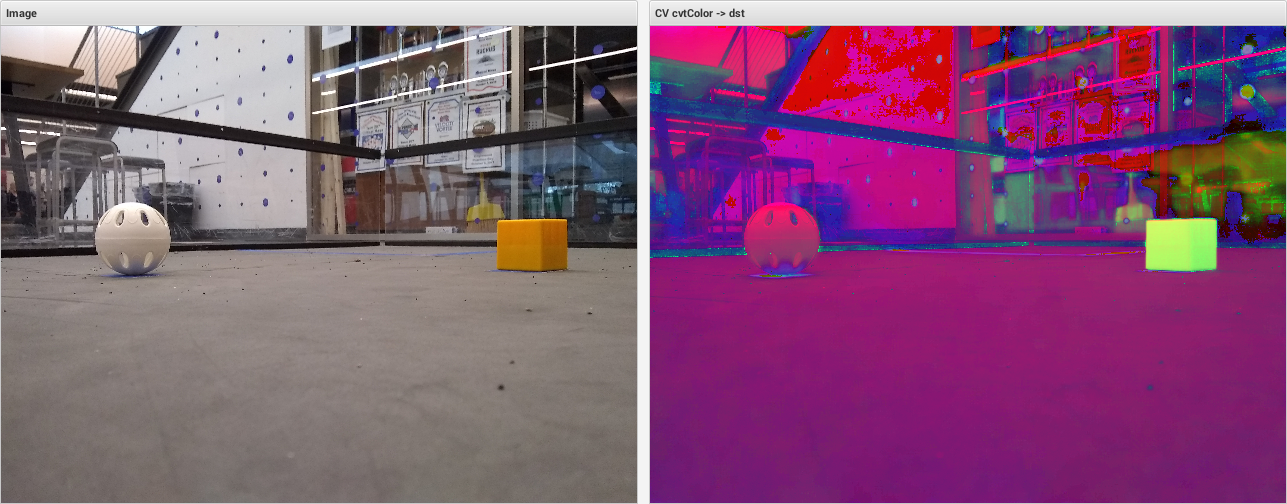
\includegraphics[width=400pt]{sections/vision/images/opencv/gold_pipeline_cvtColor.png}
    \caption{Comparison of RGB to HSV image}
\end{figure}
This is a fairly standard step, especially useful for the gold mineral as can be seen in the neon green color. The next step that we are going to perform is a blur. We do this to ensure that the edges are smoothed out. 
\begin{figure}[H]
    \centering
    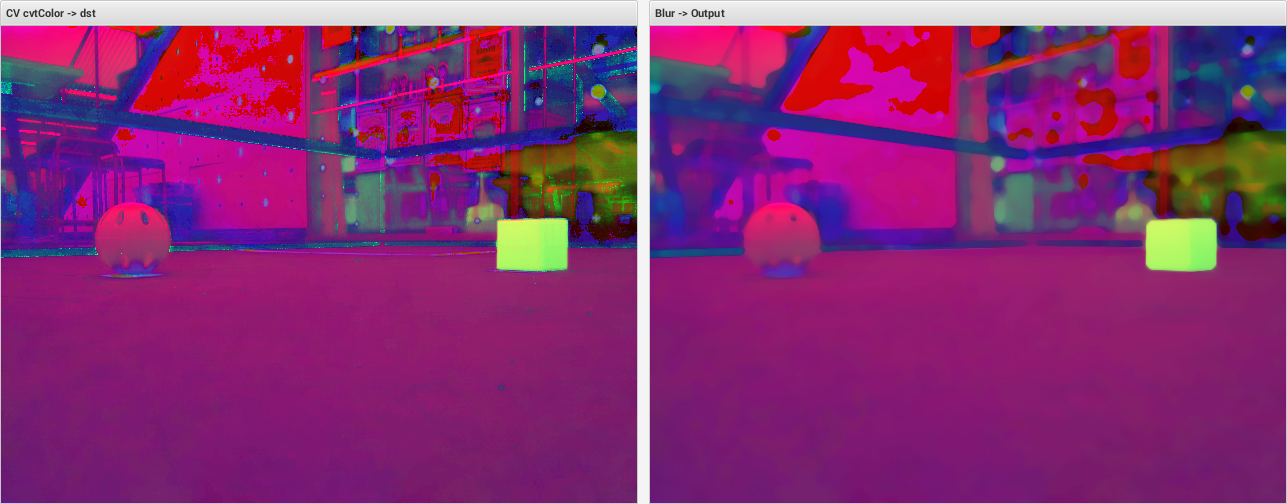
\includegraphics[width=400pt]{sections/vision/images/opencv/gold_pipeline_blur.png}
    \caption{Comparison of Pre-Blur to Post-Blur image}
\end{figure}

The next step is the ``meat and potatoes'' of the algorithm. Experimentally, we determine the range in which the color values of the gold mineral lay. Once this range is found, we perform a threshold on the image, selecting pixels which lie in that range exactly. 
\begin{figure}[H]
    \centering
    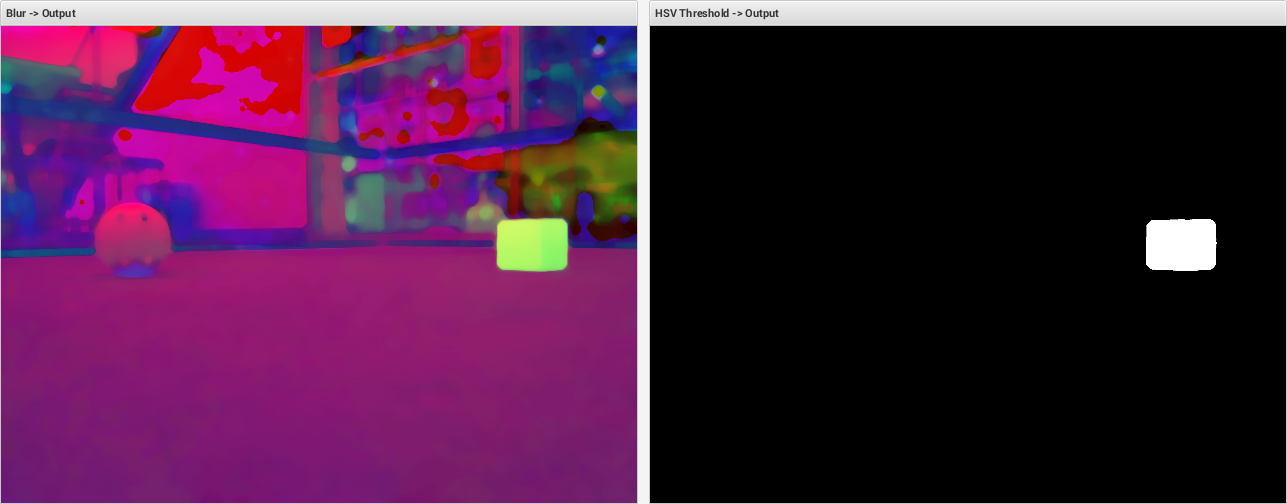
\includegraphics[width=400pt]{sections/vision/images/opencv/gold_pipeline_threshold.png}
    \caption{Comparison of Source to thresholded image}
\end{figure}

Once we have that binary image, we can run either contour detection, or blob detection. We personally recommend contours - they are faster, as well as more robust dude to the tendency of blobs to detect only blobbish objects. In this specific image, both work. However, other images in testing did not work with blobs.
\begin{figure}[H]
    \centering
    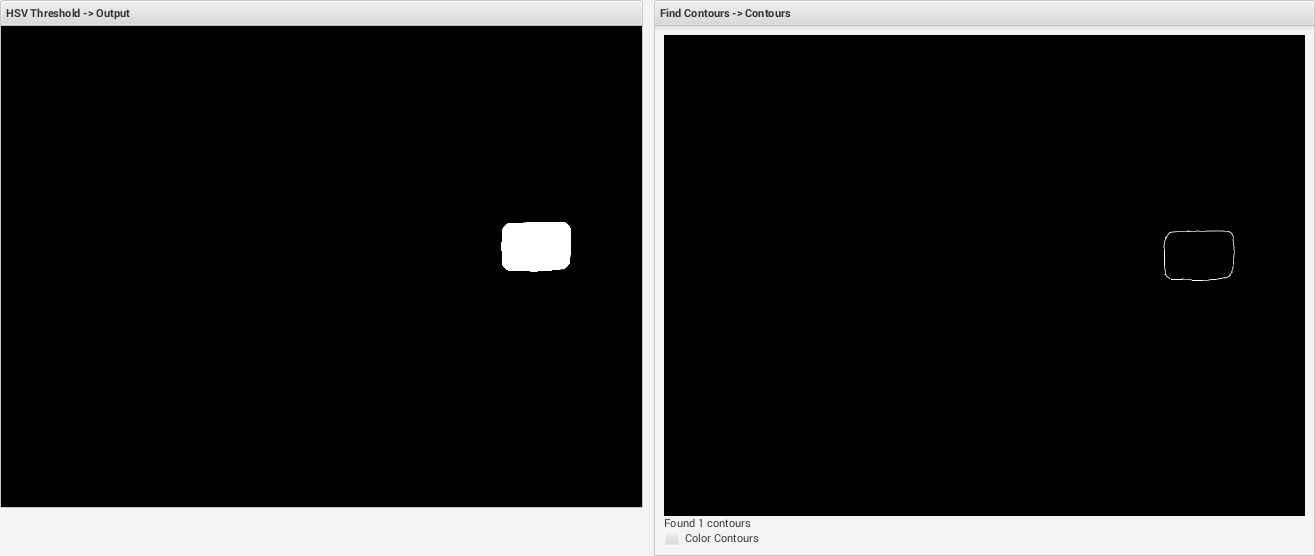
\includegraphics[width=400pt]{sections/vision/images/opencv/gold_pipeline_contour.png}
    \caption{Comparison of Source to Identified Contours. The contour line has been drawn over so you can actually see it}
\end{figure}
\begin{figure}[H]
    \centering
    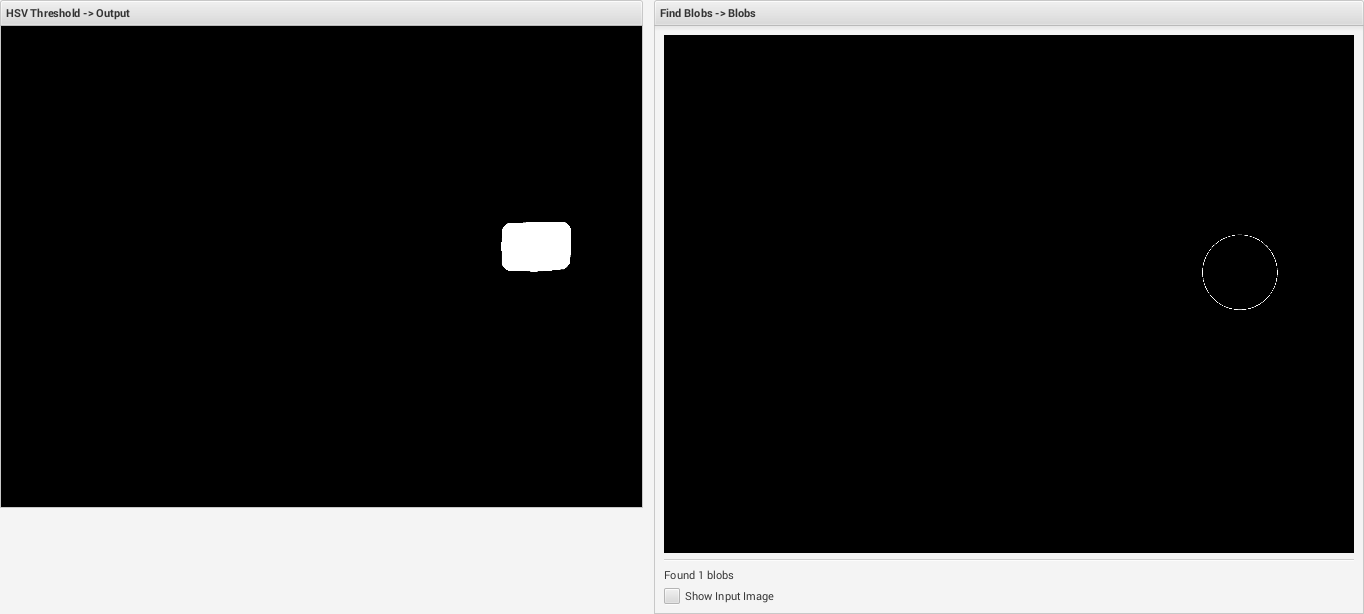
\includegraphics[width=400pt]{sections/vision/images/opencv/gold_pipeline_blob.png}
    \caption{Comparison of Source to Identified Blobs}
\end{figure}

The pipeline described above can work for a wide variety of objects. The jewels in Relic Recovery could be found in a very similar way. This pipeline is useful for identifying a small object from an image, with a uniform color across the object. When developing these types of pipelines, blurring and thresholding are very easy to mess around with to increase the efficacy of the algorithm.
\subsubsection{Silver Mineral Location Detection in the Crater in Rover Ruckus}
In this section, we will explore a OpenCV pipeline that can identify the location of silver minerals in the crater. The important note here is that the minerals are very close together, which is different from the sampling pipeline.
\begin{figure}[H]
    \centering
    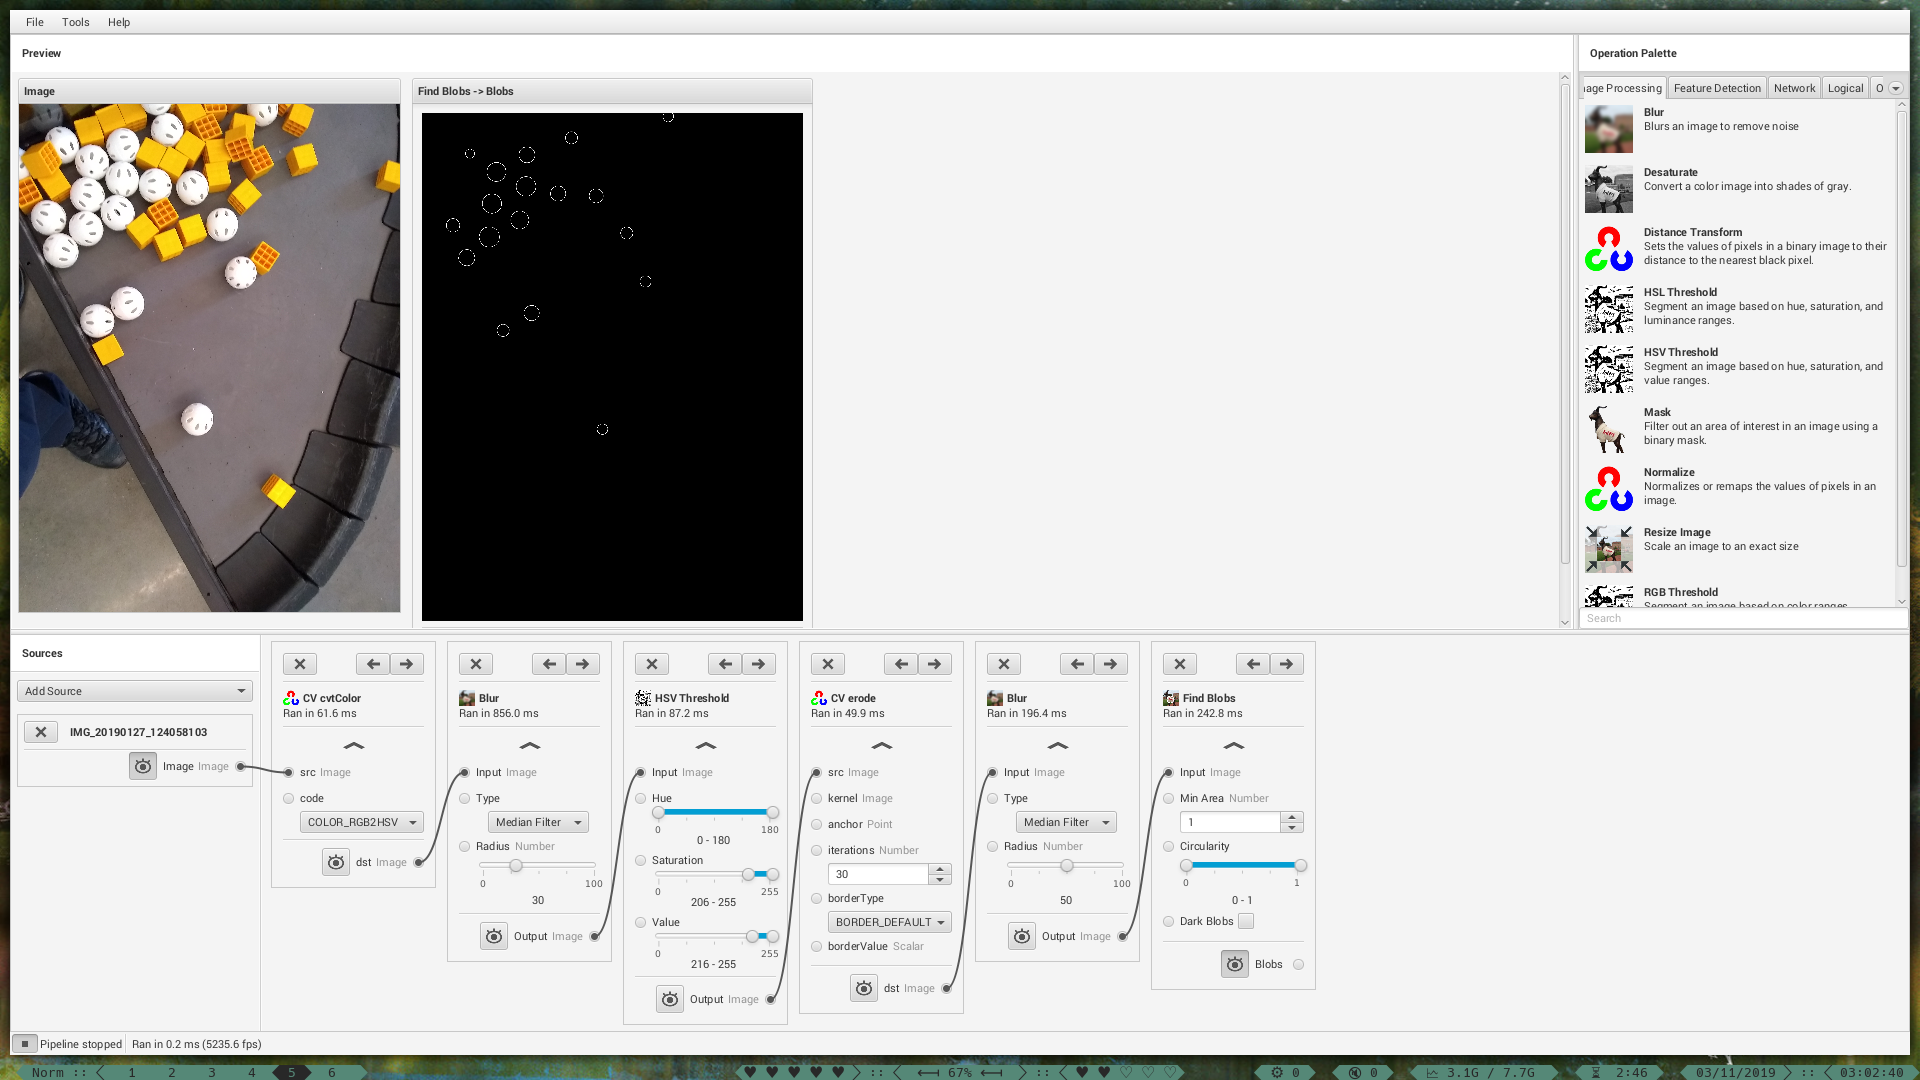
\includegraphics[width=400pt]{sections/vision/images/opencv/crater_grip_screenshot.png}
    \caption{Screenshot of the finalized pipeline, and the identified locations of the silver mineral}
\end{figure}
\subsubsection{Glyph Detection in the Pit for Relic Recovery}
\subsection{Programming OpenCV}
\subsubsection{DogeCV}
\subsubsection{EnderCV}
\subsubsection{Autogenerated GRIP Code}
\subsubsection{Example Implementation}
\inputminted[breaklines, fontsize=\small]{java}{sections/vision/code/GoldDetectorPipeline.java}
\inputminted[breaklines, fontsize=\small]{java}{sections/vision/code/GoldDetectorWrapper.java}



















\end{document}
